\documentclass[12pt]{article}
\usepackage[english]{babel}
\usepackage[utf8]{inputenc}



%% Pointer to 'default' preamble
% pacakages and definitions

\usepackage{geometry}
\geometry{
	letterpaper, 
	portrait, 
	top=.75in,
	left=.8in,
	right=.75in,
	bottom=.5in		} 	% Page Margins
	
%% additional packages for nice things
\usepackage{amsmath} 	% for most math
\usepackage{commath} 	% for abs
\usepackage{lastpage}	% for page count
\usepackage{amssymb} 	% for therefore
\usepackage{graphicx} 	% for image handling
\usepackage{wrapfig} 	% wrap figures
\usepackage[none]{hyphenat} % for no hyphenations
\usepackage{array} 		% for >{} column characterisctis
\usepackage{physics} 	% for easier derivative \dv....
\usepackage{tikz} 		% for graphic@!
\usepackage{circuitikz} % for circuits!
\usetikzlibrary{arrows.meta} % for loads
\usepackage[thicklines]{cancel}	% for cancels
\usepackage{xcolor}		% for color cancels
\usepackage[per-mode=fraction]{siunitx} % for si units and num
\sisetup{group-separator = {,}, group-minimum-digits = 3} % additional si unit table functionality

\usepackage{fancyhdr} 	% for header
\usepackage{comment}	% for ability to comment out large sections
\usepackage{multicol}	% for multiple columns using multicols
\usepackage[framed,numbered]{matlab-prettifier} % matlab sytle listing
\usepackage{marvosym} 	% for boltsymbol lightning
\usepackage{pdflscape} 	% for various landscape pages in portrait docs.
%\usepackage{float}
\usepackage{fancyvrb}	% for Verbatim (a tab respecting verbatim)
\usepackage{enumitem}	% for [resume] functionality of enumerate
\usepackage{spreadtab} 	% for using formulas in tables}
\usepackage{numprint}	% for number format in spread tab
\usepackage{subcaption} % for subfigures with captions
\usepackage[normalem]{ulem} % for strike through sout

% for row colors in tables....
\usepackage{color, colortbl}
\definecolor{G1}{gray}{0.9}
\definecolor{G2}{rgb}{1,0.88,1}%{gray}{0.6}
\definecolor{G3}{rgb}{0.88,1,1}

% For table formatting
\usepackage{booktabs}
\renewcommand{\arraystretch}{1.2}
\usepackage{floatrow}
\floatsetup[table]{capposition=top} % put table captions on top of tables

% Caption formating footnotesize ~ 10 pt in a 12 pt document
\usepackage[font={small}]{caption}

%% package config 
\sisetup{output-exponent-marker=\ensuremath{\mathrm{E}}} % for engineer E
\renewcommand{\CancelColor}{\color{red}}	% for color cancels
\lstset{aboveskip=2pt,belowskip=2pt} % for more compact table
%\arraycolsep=1.4pt\def
\setlength{\parindent}{0cm} % Remove indentation from paragraphs
\setlength{\columnsep}{0.5cm}
\lstset{
	style      = Matlab-editor,
	basicstyle = \ttfamily\footnotesize, % if you want to use Courier - not really used?
}
\renewcommand*{\pd}[3][]{\ensuremath{\dfrac{\partial^{#1} #2}{\partial #3}}} % for larger pd fracs
\renewcommand{\real}[1]{\mathbb{R}\left\{ #1 \right\}}	% for REAL symbol
\newcommand{\imag}[1]{\mathbb{I}\left\{ #1 \right\}}	% for IMAG symbol
\definecolor{m}{rgb}{1,0,1}	% for MATLAB matching magenta
	
%% custom macros
\newcommand\numberthis{\addtocounter{equation}{1}\tag{\theequation}} % for simple \numberthis command

\newcommand{\equal}{=} % so circuitikz can have an = in the labels
\newcolumntype{L}[1]{>{\raggedright\let\newline\\\arraybackslash\hspace{0pt}}m{#1}}
\newcolumntype{C}[1]{>{\centering\let\newline\\\arraybackslash\hspace{0pt}}m{#1}}
\newcolumntype{R}[1]{>{\raggedleft\let\newline\\\arraybackslash\hspace{0pt}}m{#1}}

%% Header
\pagestyle{fancy} % for header stuffs
\fancyhf{}
% spacing
\headheight 29 pt
\headsep 6 pt

%% Header
\rhead{Thad Haines \\ Page \thepage\ of \pageref{LastPage}}
\chead{PST and AGC \\ }
\lhead{Research \\ 7/20/20}
\usepackage{minted}
\usepackage{setspace}
\begin{document}
\onehalfspacing
\paragraph{Purpose} \ \\
This document is meant to explain PST additions and alterations created to accommodate AGC.
Code examples are taken from the AGC example file \verb|d2a_AGC.m| which is a modified version of \verb|d2a_dce.m|.


\paragraph{Area Definitions} \ \\
To enable area calculations, each bus  in the \verb|bus| array must be assigned to an area in the \verb|area_def| array.
An example \verb|area_def| array is shown below.
\begin{minted}[
		frame=lines,
		framesep=2mm,
		baselinestretch=1.2,
		bgcolor=gray!13,
		fontsize=\footnotesize,
		%linenos,
		breaklines
		]{MATLAB}
%% area_def data format
% should contain same number of rows as bus array (i.e. all bus areas defined)
% col 1 bus number
% col 2 area number
area_def = [ ...
            1  1;
            2  1;
            3  1;
            4  1;
            10 1;
            11 2;
            12 2;
            13 2;
            14 2; 
            20 1;
           101 1; 
           110 2;
           120 2];
\end{minted}

It should be noted that rows may not have to be in the same order as the bus array (untested).
The \verb|area_def| array is automatically placed into the global g structure.
\begin{minted}[
		frame=lines,
		framesep=2mm,
		baselinestretch=1.2,
		bgcolor=gray!13,
		fontsize=\footnotesize,
		%linenos,
		breaklines
		]{MATLAB}
>> g.area
ans = 
    area_def: [13x2 double]
      n_area: 2
        area: [1x2 struct]
\end{minted}

Each area currently contains values that may be relevant to AGC calculations.
The \verb|calcAreaVals| function is used to calculate and store such values.
An example of what is stored in the \verb|g.area.area(x)| structure is shown below.
\pagebreak
\begin{minted}[
		frame=lines,
		framesep=2mm,
		baselinestretch=1.2,
		bgcolor=gray!13,
		fontsize=\footnotesize,
		%linenos,
		breaklines
		]{MATLAB}
>> g.area.area(2)
ans = 
         number: 2
      areaBuses: [6x1 double]
         macBus: [2x1 double]
      macBusNdx: [3 4]
        loadBus: [4x1 double]
     loadBusNdx: [8 9 12 13]
         genBus: [2x1 double]
      genBusNdx: [6 7]
           totH: [1x4063 double]
           aveF: [1x4063 double]
         totGen: [1x4063 double]
        totLoad: []
            icA: [1x4063 double]
            icS: []
  exportLineNdx: [11 12]
  importLineNdx: []
       n_export: 2
       n_import: []
\end{minted}
It should be noted that \verb|icS| represents a placeholder for a scheduled interchange value and the \verb|totLoad|  is a field for collected total load.
The collection of actual running load values may prove more complicated as the bus array does not seem to be updated every step, only a reduced Y matrix used in the \verb|nc_load| function called from \verb|i_simu|. 
 
 \pagebreak
\paragraph{Line Monitoring} \ \\
Power flow on a line must be calculated each step as AGC requires actual area interchange for the ACE calculation.
The previously existing \verb|line_pq| function performed this task, but was not fully implemented into the simulation to allow calculation during execution.
This minor oversight has been resolved and the \verb|lmon_con| array is still used to define monitored lines as in previous version of PST.

\begin{minted}[
		frame=lines,
		framesep=2mm,
		baselinestretch=1.2,
		bgcolor=gray!13,
		fontsize=\footnotesize,
		%linenos,
		breaklines
		]{MATLAB}
%% Line Monitoring
% Each value corresponds to an array index in the line array.
% Complex current and power flow on the line will be calculated and logged during simulation

%lmon_con = [5, 6, 13]; % lines between bus 3 and 101, and line between 13 and 120

lmon_con = [3,10]; % lines to loads
\end{minted}

Line monitoring data is collected in the \verb|g.lmon| field of the global variable.

\begin{minted}[
		frame=lines,
		framesep=2mm,
		baselinestretch=1.2,
		bgcolor=gray!13,
		fontsize=\footnotesize,
		%linenos,
		breaklines
		]{MATLAB}
>> g.lmon
ans = 
     lmon_con: [3 10]
       n_lmon: 2
    busFromTo: [2x2 double]
         line: [1x2 struct]
\end{minted}

Each \verb|g.lmon.line| entry contains the following fields and logged data:

\begin{minted}[
		frame=lines,
		framesep=2mm,
		baselinestretch=1.2,
		bgcolor=gray!13,
		fontsize=\footnotesize,
		%linenos,
		breaklines
		]{MATLAB}
>> g.lmon.line(2)
ans = 
    busArrayNdx: 10
        FromBus: 13
          ToBus: 14
          iFrom: [1x4063 double]
            iTo: [1x4063 double]
          sFrom: [1x4063 double]
            sTo: [1x4063 double]
\end{minted}

\pagebreak
\paragraph{Weighted Average Frequency} \ \\
An average weighted frequency is calculated for the total system and for each area if there are areas detected.
The calculation involves a sum of system inertias that may change with generator trips.
The current algorithm does not account for tripped generators, but was designed to incorporate this feature in the future.

\vspace{1em}
In a system with $N$ generators, $M$ areas, and $N_M$ generators in area $M$, the \verb|calcAveF| function performs the following calculations for each area $M$:

\begin{align*}
%         % calculate weighted average frequency for each area, sum for system
%         runningSysF = 0;
%         runningSysH = 0;
%         for areaN=1:g.area.n_area
%             % calculate area total inertia
%             mNdx = g.area.area(areaN).macBusNdx;
%             g.area.area(areaN).totH(k) = sum(g.mac.mac_con(mNdx,16).*g.mac.mac_con(mNdx,3));
%             % calculate ave weighted f = sum(mac_speed.*MVA.*H) / totH
%             g.area.area(areaN).aveF(k) = sum(g.mac.mac_spd(mNdx,k).*g.mac.mac_con(mNdx,3).*g.mac.mac_con(mNdx,16)) ...
%                 /g.area.area(areaN).totH(k);
%             
%             runningSysF = runningSysF + g.area.area(areaN).aveF(k);
%             runningSysH = runningSysH + g.area.area(areaN).totH(k);
%         end
%         
%         %g.sys.totH(k) = sum(g.mac.mac_con(:,16).*g.mac.mac_con(:,3));
%         g.sys.totH(k) = runningSysH;
%         g.sys.aveF(k) = runningSysF/g.area.n_area;
H_{tot_M} &= \sum_{i}^{N_M} MVA_{base_i}H_i \\
F_{ave_M} &= \left( \sum_{i}^{N_M}Mach_{speed_i}MVA_{base_i}H_i \right) \dfrac{1}{H_{tot_M}}
\end{align*}

Then system total values are calculated as
\begin{align*}
H_{tot} &= \sum_{i}^{M} H_{tot_M} \\
F_{ave} &= \left( \sum_{i}^{M} F_{ave_M} \right) \dfrac{1}{M}
\end{align*}

If $M==0$, \verb|calcAveF| performs
\begin{align*}
H_{tot} &= \sum_{i}^{N} MVA_{base_i}H_i \\
F_{ave} &= \left( \sum_{i}^{N}Mach_{speed_i}MVA_{base_i}H_i \right) \dfrac{1}{H_{tot}}
\end{align*}

\pagebreak
\paragraph{Automatic Generation Control} \ \\
RACE and SACE are calculated using PU values assuming B is a positive non-PU value with units of $MW/0.1Hz$
If $K_{bv}$ is not zero, the resulting $RACE$ is not the industry standard $RACE$ value.
\begin{center}
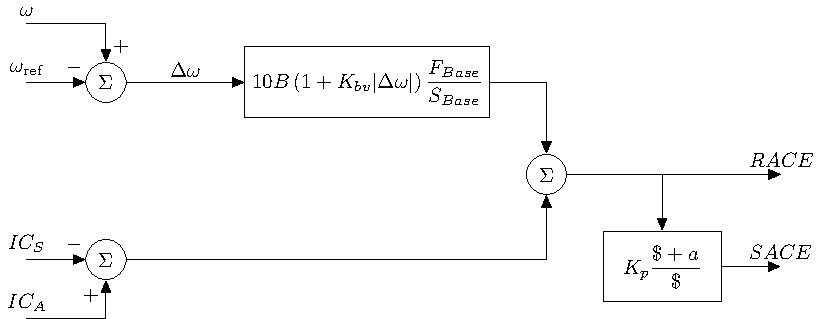
\includegraphics[width=.8\linewidth]{200722-AGCblockdiagram-p1}
\end{center}

The action of the AGC model is determined by the \verb|startTime| and \verb|actionTime| variables.
Assuming action, the conditional $\Delta\omega$ logic is processed before adjusting the \verb|aceSig| value which is then gained to become \verb|ace2dist|.

\begin{center}
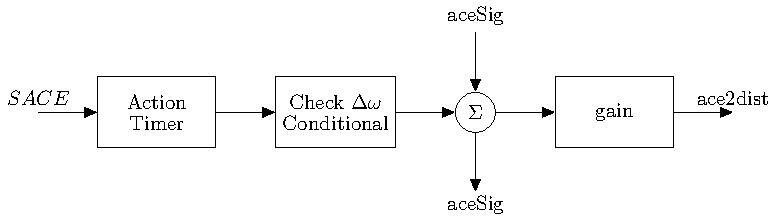
\includegraphics[width=.8\linewidth]{200722-AGCblockdiagram-p2}
\end{center}

The \verb|ace2dist| value is distributed to all controlled generators according to their respective participation factor \verb|pF|.
Each \verb|ctrlGen| has a unique low pass filter that processes the signal that is then gained by -1 and added to the existing associated governor \verb|tg_sig| value.

\begin{center}
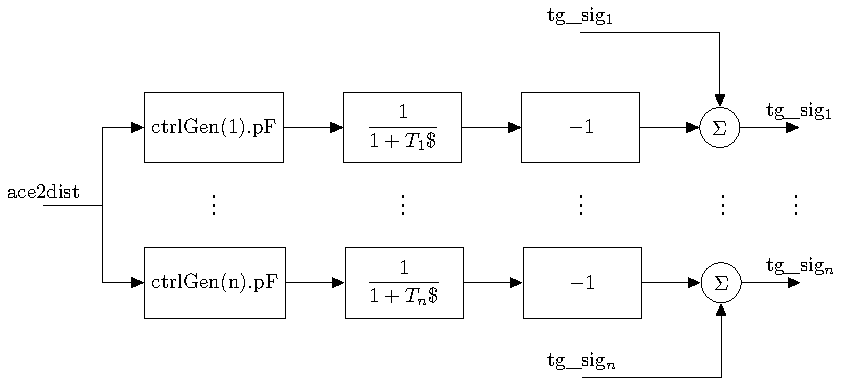
\includegraphics[width=.85\linewidth]{200722-AGCblockdiagram-p3}
\end{center}
\pagebreak
\paragraph{Example AGC settings} \ \\ 
The following AGC settings are not entirely realistic, but useful in demonstrating the required user definitions and functionality of the AGC model.

\begin{minted}[
		frame=lines,
		framesep=2mm,
		baselinestretch=1.2,
		bgcolor=gray!13,
		fontsize=\footnotesize,
		%linenos,
		breaklines
		]{MATLAB}
%% AGC definition

%{ 
Experimental model definition akin to Trudnowski experimental code.
Each agc(x) has following fields:
    area        - Area number / controlled area
    startTime   - Time of first AGC signal to send
    actionTime  - Interval of time between all following AGC signals
    gain        - Gain of output ACE signal
    Btype       - Fixed frequency bias type (abs, percent of max capacity...)
        0 - absolute - Input B value is set as Frequency bias (positive MW/0.1Hz)
        1 - percent of max area capacity
    B           - Fixed frequency bias Value
    Kbv         - Varaible frequency bias gain used to gain B as B(1+kBv*abs(delta_w))
    condAce     - Conditional ACE flag
        0 - Conditional ACE not considered
        1 - ace2dist updated only if sign matches delta_w (i.e. in area event)

    (PI Filter Values)
    Kp          - Proportional gain
    a           - ratio between integral and proportional gain (placement of zero)

    ctrlGen_con - Controlled generator information (see format note below)
%}

agc(1).area = 1;
agc(1).startTime = 25;
agc(1).actionTime = 15;
agc(1).gain = 2; % gain of output signal
agc(1).Btype = 1; % per max area capacity
agc(1).B = 1;
agc(1).Kbv = 0; % no variable bias
agc(1).condAce = 0; % conditional ACE
agc(1).Kp = 0.04;
agc(1).a = 0.001;
agc(1).ctrlGen_con = [ ...
    % ctrlGen_con Format:
    %col 1 gen bus
    %col 2 participation Factor
    %col 3 low pass filter time constant [seconds]
    1, 0.75, 15;
    2, 0.25, 2;
    ];

agc(2)=agc(1); % duplicate most settings from AGC 1 to AGC 2
agc(2).area = 2;
agc(2).ctrlGen_con = [...
%    col 1 gen bus
%    col 2 participation Factor
    %col 3 low pass filter time constant [seconds]
    11, 0.25, 10;
    12, 0.75, 5;
    ];
\end{minted}

%\pagebreak
\paragraph{General Example Scenario Details} \ \\

\begin{center}
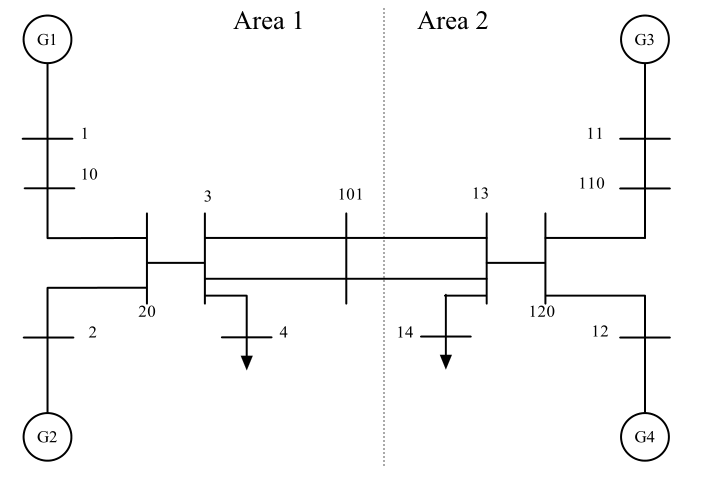
\includegraphics[width=.75\linewidth]{sysOneLineAreas}
\end{center}
\begin{itemize}
\item Kundur  4 machine system packaged with PST
\item Constant Z load model
\item All machines, exciters, and govs identical
\item PSS on gen 1 and 3
\item SVC on bus 101
\item Event: +50 MW (0.5 PU) step of load on bus 4 at t=1
\item AGC model available in pstSETO only
\end{itemize}

\pagebreak
\paragraph{Initial simulation results (No AGC)} \ \\


\begin{center}
\newcommand{\caseName}{NoAGC}
\includegraphics[width=.45\linewidth]{\caseName f1} %
\includegraphics[width=.45\linewidth]{\caseName f2} \\%
\includegraphics[width=.45\linewidth]{\caseName f3} %
\includegraphics[width=.45\linewidth]{\caseName f4} \\%
\includegraphics[width=.45\linewidth]{\caseName f5} %
\includegraphics[width=.45\linewidth]{\caseName f6} \\%
\end{center}

\pagebreak
\paragraph{Initial simulation results (with AGC)} \ \\

\begin{center}
\newcommand{\caseName}{AGC}
\includegraphics[width=.45\linewidth]{\caseName f4} %
\includegraphics[width=.45\linewidth]{\caseName f2} \\%
\includegraphics[width=.45\linewidth]{\caseName f3} %
\includegraphics[width=.45\linewidth]{\caseName f5} \\%
\includegraphics[width=.45\linewidth]{\caseName f6} %
\includegraphics[width=.45\linewidth]{\caseName f7} \\%
\end{center}

\pagebreak
\paragraph{Initial simulation results (with conditional AGC)} \ \\


\begin{center}
\newcommand{\caseName}{AGCcond}
\includegraphics[width=.45\linewidth]{\caseName f4} %
\includegraphics[width=.45\linewidth]{\caseName f2} \\%
\includegraphics[width=.45\linewidth]{\caseName f3} %
\includegraphics[width=.45\linewidth]{\caseName f5} \\%
\includegraphics[width=.45\linewidth]{\caseName f6} %
\includegraphics[width=.45\linewidth]{\caseName f7} \\%
\end{center}
\begin{comment}


\begin{minted}[
		frame=lines,
		framesep=2mm,
		baselinestretch=1.2,
		bgcolor=gray!13,
		fontsize=\footnotesize,
	%	linenos,
		breaklines
				]{MATLAB}
XxXxX

\end{minted}

\end{comment}


\end{document}
